% !TEX TS-program = pdflatex
% !TEX encoding = UTF-8 Unicode

% This is a simple template for a LaTeX document using the "article" class.
% See "book", "report", "letter" for other types of document.

\documentclass[11pt]{article} % use larger type; default would be 10pt

\usepackage[utf8]{inputenc} % set input encoding (not needed with XeLaTeX)

%%% Examples of Article customizations
% These packages are optional, depending whether you want the features they provide.
% See the LaTeX Companion or other references for full information.

%%% PAGE DIMENSIONS
\usepackage{geometry} % to change the page dimensions
\geometry{a4paper} % or letterpaper (US) or a5paper or....
% \geometry{margin=2in} % for example, change the margins to 2 inches all round
% \geometry{landscape} % set up the page for landscape
%   read geometry.pdf for detailed page layout information

\usepackage{graphicx} % support the \includegraphics command and options

% \usepackage[parfill]{parskip} % Activate to begin paragraphs with an empty line rather than an indent

%%% PACKAGES
\usepackage{booktabs} % for much better looking tables
\usepackage{array} % for better arrays (eg matrices) in maths
\usepackage{paralist} % very flexible & customisable lists (eg. enumerate/itemize, etc.)
\usepackage{verbatim} % adds environment for commenting out blocks of text & for better verbatim
\usepackage{subfig} % make it possible to include more than one captioned figure/table in a single float
% These packages are all incorporated in the memoir class to one degree or another...

%%% HEADERS & FOOTERS
\usepackage{fancyhdr} % This should be set AFTER setting up the page geometry
\pagestyle{fancy} % options: empty , plain , fancy
\renewcommand{\headrulewidth}{0pt} % customise the layout...
\lhead{}\chead{}\rhead{}
\lfoot{}\cfoot{\thepage}\rfoot{}

%%% SECTION TITLE APPEARANCE
\usepackage{sectsty}
\allsectionsfont{\sffamily\mdseries\upshape} % (See the fntguide.pdf for font help)
% (This matches ConTeXt defaults)

%%% ToC (table of contents) APPEARANCE
\usepackage[nottoc,notlof,notlot]{tocbibind} % Put the bibliography in the ToC
\usepackage[titles,subfigure]{tocloft} % Alter the style of the Table of Contents
\renewcommand{\cftsecfont}{\rmfamily\mdseries\upshape}
\renewcommand{\cftsecpagefont}{\rmfamily\mdseries\upshape} % No bold!

%%% END Article customizations

\usepackage[spanish]{babel}
\usepackage{listings} 
%%% The "real" document content comes below...


\title{\fontsize{30}{0} \bf BUSCAMINAS}
\author{\\Autores: \\  \\-Cristina Barreno \\ -Sixto Castro \\ -Jordy Vasquez\\ \\}
\thispagestyle{empty}
\begin{document}

\newpage

 
\includegraphics[width=3cm]{./imagenes/Espol.png}{ \fontsize{18}{0} \bf ESCUELA SUPERIOR \\}
\begin{center}
{\fontsize{18}{0} \bf POLITÉCNICA DEL LITORAL\\}
\vspace{2cm}
{\LARGE{ DOCUMENTACIÓN DEL BUSCAMINAS }}\\
\vspace{2cm}
{\LARGE{ Materia: Lenguajes de Programación }}\\
\vspace{2cm}
{\LARGE{ Paralelo: 1}}\\
\vspace{2cm}
{\LARGE{Fecha de entrega: \\  Miércoles, 11 de Diciembre del 2013}}
\thispagestyle{empty}
\end{center}


\maketitle

\newpage
\tableofcontents % No hace falta un TOC en un artículo corto
\thispagestyle{empty}
\addtocontents{toc}{\protect\thispagestyle{empty}}

\newpage
\begin{center}
 {\fontsize{16}{0} \bf Documentación del Proyecto Buscaminas}
\end{center}

\section{\fontsize{14}{0} \bf Introducción}
\section{\fontsize{14}{0} \bf Justificación}
\section{\fontsize{14}{0} \bf Desarrollo}
\section{\fontsize{14}{0} \bf Alcances}
\section{\fontsize{14}{0} \bf Manual}
\begin{itemize}
 \item Este juego consiste en destapar todas las casillas que no oculten una mina.\\
 \item Algunas casillas tienen un número, el cual nos indica el total de minas que se encuentran alrededor de esa casilla. Por Ej: Si una casilla tiene el número 6, significa que de las ocho casillas que hay alrededor de aquella casilla marcada (si no es en una esquina o borde) hay 6 con minas y 2 sin minas. Si se descubre una casilla sin número indica que ninguna de las casillas vecinas tiene mina y estas se van a descubrir (destapar) automáticamente.\\
 \item Si se descubre una casilla con una mina se pierde la partida.\\
 \item Se puede poner una bandera en las casillas donde el jugador piensa que hay minas para ayudar a descubrir aquellas que tienen minas.\\
 \item El juego también posee un sistema de récords para cada nivel en el que se muestra los usuarios que han ganado en el menor tiempo posible. Los niveles son:\\
\begin{itemize}
 \item Nivel principiante: 8 x 8 casillas y 10 minas.
 \item Nivel intermedio: 16 x 16 casillas y 40 minas.
 \item Nivel experto: 16 x 20 casillas y 60 minas.

\end{itemize}
\end{itemize}

\newpage
\section{\fontsize{14}{0} \bf Imágenes}
\begin{itemize}
\item {\bf Menú principal}\\\\\\\\
 \centerline{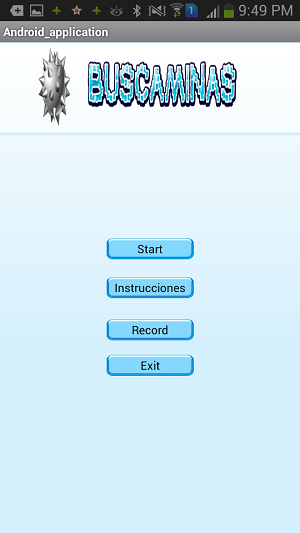
\includegraphics[width=0.5\textwidth]{./imagenes/Menu}}\\
\newpage
\item {\bf Jugar}\\\\
Cuenta con varios niveles: Fácil, intermedio y difícil.
\begin{itemize}
\item {\bf Nivel fácil}\\\\
  \centerline{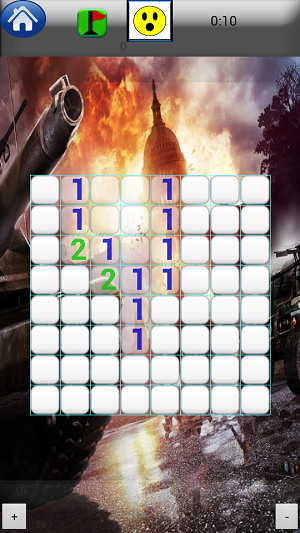
\includegraphics[width=0.5\textwidth]{./imagenes/Nivelfacil}}
\newpage
\item {\bf Nivel intermedio}\\\\\\\\
  \centerline{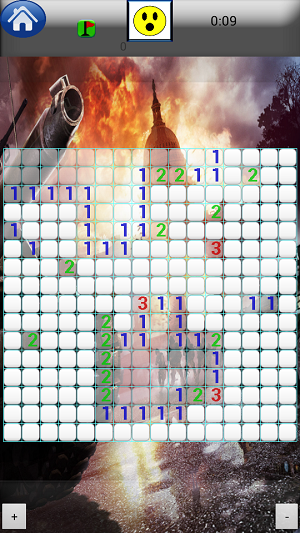
\includegraphics[width=0.5\textwidth]{./imagenes/Nivelintermedio}}
\newpage
\item {\bf Nivel difícil}\\\\\\\\
 \centerline{ 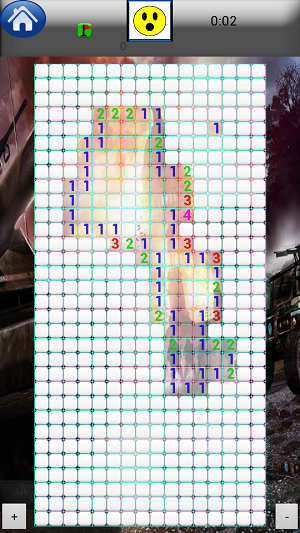
\includegraphics[width=0.5\textwidth]{./imagenes/Niveldificil}}
\end{itemize}
\newpage
\item {\bf Gana}\\\\\\
Se muestra una cara feliz con gafas indicando que uno ha ganado. Además se presenta un pantalla mostrando el tiempo en que ganó el usuario, también le pide el nombre del usuario para guardarlo en la base de datos (Records).\\\\
  \centerline{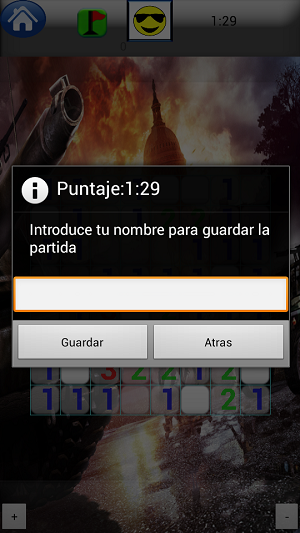
\includegraphics[width=0.5\textwidth]{./imagenes/ganar}}
\newpage
\item {\bf Records}\\\\\\\\
 \centerline{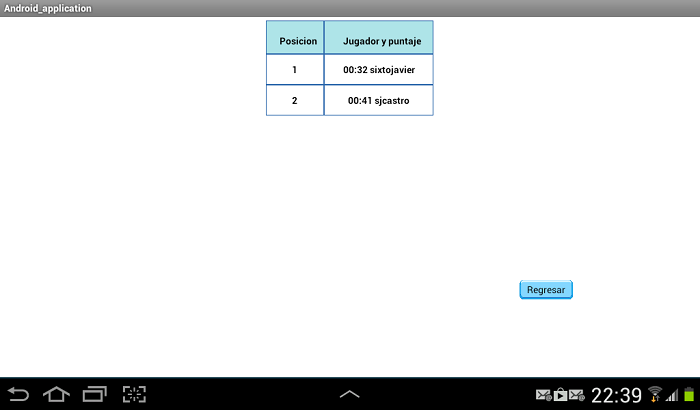
\includegraphics[width=0.8\textwidth]{./imagenes/Records}}
\newpage
\item {\bf Instrucciones}\\\\\\\\
 \centerline{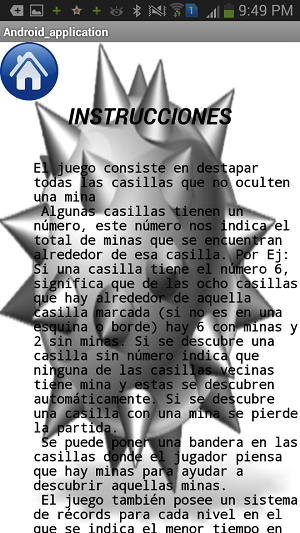
\includegraphics[width=0.5\textwidth]{./imagenes/Instrucciones}}


\end{itemize}

\section{\fontsize{14}{0} \bf Observaciones}
\section{\fontsize{14}{0} \bf Conclusiones}

\end{document}
